
\documentclass[11pt]{report}


\usepackage[pdftex]{graphicx}
\usepackage{url} 
\usepackage[dvips, bookmarks, colorlinks=false, pdfborder={0 0 0}, pdftitle={<pdf title here>}, pdfauthor={<author's name here>}, pdfsubject={<subject here>}, pdfkeywords={<keywords here>}]{hyperref} 
\usepackage[final]{pdfpages}
\usepackage{multirow}
\usepackage[table]{xcolor} 
\usepackage{subfigure}
\usepackage{booktabs}


\newtheorem{example}{Example}[section]
\newtheorem{defn}{Def}
\newcommand{\ESIM}{\textsc{E}\small{\texttt{SIM}}~}
\newcommand\T{\rule{0pt}{3.1ex}}		% To add space b/w words and top \hline
\renewcommand{\figurename}{Fig.}

\newcommand\counter[1]{\arabic{#1} \stepcounter{#1}}
\newcounter{syscall}
\title{XSM \\ eXperimental String Machine \\
Version 1.0}
\author{Dr. K. Muralikrishnan  \\ \texttt{kmurali@nitc.ac.in} \\ {NIT Calicut} }


\begin{document}

\maketitle
\pagebreak

%......................Table of Contents............................%
\thispagestyle{plain}

\tableofcontents
\pagebreak

\chapter{Introduction}
\label{chp:osintro}
%The OS provides an interface to the user to interact with the hardware. Users write programs that make use of various resources like disk, memory, processor etc. These programs are run as processes on the machine.
%
%The system programmers use the language SP-SIL for writing the Operating System. User programs to test the various functionalities of the Operating System can be written in AP-SIL. Refer the documents ~\cite{spsil} and ~\cite{apsil} for the complete documentation of these tools.
%
%A detailed operating system specification was done in the works of ~\cite{group1} and ~\cite{group2}. This documentation was critically reviewed and modifications were done in many places to comply with our new design.
%The major modifications done are the following:
%\begin{itemize}
%\item Introduction of INIT process (refer section \ref{lbl:INITprocess})
%\item Introduction of Halt() system call (refer chapter \ref{chp:halt_system_calls})
%\item Exception handler interrupt has been excluded due to some limitations in the design.
%\item The distribution of system calls were changed. This was due to the limitations in interrupt code size.
%\end{itemize}

\section{Operating System Functionality}
There are various functionalities associated with the operating system which are essential for the user programs to run and make use of the system resources. The functionalities and their details are explained below.

\subsection{Process Management}
Any program that the user wishes to execute is loaded into the memory (A program in memory is known as a process). For creating a new process,


\subsection{Multiprogramming}
The operating system allows multiple processes to be run on the machine and manages the system resources among these processes. 
This process of simultaneous execution of multiple processes is known as \emph{multiprogramming}. Refer chapter~\ref{chp:multiprog} to know more about multiprogramming.

\subsection{System Calls}
A process needs resources like disk, memory etc while executing. The OS caters to these needs of the process by providing an interface  known as the \emph{system call interface}. Refer chapter~\ref{chp:file_system_calls} and chapter~\ref{chp:process_system_calls} to know more about system calls.

%\section{Exception Handling}
%Whenever the machine deviates from its normal execution, an exception occurs. To handle this exception, machine generates the 
%interrupt corresponding to exception handling (\texttt{INT 7}). The exception handler restores the machine back to its normal state
%and continues the execution of the other processes. Refer chapter~\ref{chp:exception} to know more about exception handling.


\chapter{Memory}
\label{chp:memory}
\index{Memory}

\section{Introduction} 
\index{Memory!Structure}

\begin{figure}[htp!] \small
	\centering
	\begin{tabular}{|c|c|c|}
		\textbf{Page no} & \textbf{Contents} & \textbf{Word addr} \\
		0   & \hyperref[lbl:romcode]{ROM code} 		& 0 -- 255 \\ \hline 
		1   & \hyperref[lbl:oscode]{OS Startup code} 	& 256 -- 511  \\ \hline 
		\multirow{5}{*}{2} 
			& \hyperref[lbl:pgtbl]{Static Page Tables}   & 512 -- 559 \\ \cline{2-3} 
			& \hyperref[lbl:memlst]{Memory Free List}  & 560 -- 623  \\ \cline{2-3}
			& \hyperref[lbl:gft]{Global File Table}  & 624 -- 719 \\ \cline{2-3}
			& \hyperref[lbl:rdylst]{Ready List} & 720 -- 731 \\ \cline{2-3}
			& Unallocated & 732 -- 767 \\ \hline 
		\multirow{2}{*}{3}
			& \hyperref[lbl:proctbl]{Process Table} & 768 -- 959 \\ \cline{2-3}
			& Unallocated & 960 -- 1023 \\ \hline 
		4 & \multirow{2}{*}
			{\hyperref[lbl:fat]{File Allocation Table}} & \multirow{2}{*}{1024 -- 1535} \\ \cline{1-1} 
		5 & 				 &  \\ \hline 
		6 & \multirow{2}{*}
			{\hyperref[lbl:disklst]{Disk Free List}} & \multirow{2}{*}{1536 -- 2047}\\ \cline{1-1} 
		7 & 				& \\ \hline 
		8 & \multirow{3}{*}
			{\hyperref[lbl:INITprocess]{INIT process}} & \multirow{3}{*}{2048 -- 2815} \\ \cline{1-1} 
		9 & 				 &  \\ \cline{1-1} 
		10 & 				 &  \\ \hline 
		\multirow{3}{*}{11 -- 55}
			&  \vdots & \\   
			&  User Programs & 2816 -- 14335 \\  
			& \vdots & \\ \hline 
		56 & \hyperref[lbl:int]{INT 0} & 14336 -- 14591 \\ \hline 
		57 & \hyperref[lbl:int]{INT 1} & 14592 -- 14848 \\ \hline 
		\vdots & \vdots & \vdots \\ \hline 
		63 & \hyperref[lbl:int]{INT 7} & 16128 -- 16383 \\  

	\end{tabular}
	\caption{Outline of the main memory}
	\label{1}
	\index{Memory!Structure}
\end{figure}

\begin{itemize}
	\item The basic unit of memory in the \ESIM architecture is a word. \index{Memory!Word}
	\item The machine memory can be thought of as a linear sequence of words.
	\item A collection of 256 contiguous words is known as a \emph{page}. \index{Memory!Page}
	\item The total size of the memory is 64 pages or 16384 ($256 \times 64$) words.
	\item Each word in the memory is identified by the \emph{word address} in the range 0 to $16383(256 \times 64 - 1)$. Similarly, each page in the memory is identified by the \emph{page number} \index{Memory!Page number} in the range 0 to 63.
\end{itemize}

\begin{example}
	The $256^{th}$ word of the memory has a word address 255 and belongs to page 0. In general, the $n^{th}$ word has the word address $(n-1)$, where  $1 \le n \le 16384$ and belongs to the page $\lfloor \frac{n-1}{256} \rfloor$. Refer figure~\ref{fig:mem_struct}. 
\end{example}

\begin{figure}[htp!] \small
	\centering
	\begin{tabular}{c|c|c|} 
		\multicolumn{3}{c}{} \\
		\textbf{Word address} &  & \textbf{Page no.} \\ \cline{2-3}
		0 & $1^{st}$ word & \multirow{4}{*}{$0$} \\ \cline{2-2}
		1 & $2^{nd}$ word &  \\ \cline{2-2}
		\vdots & \vdots & \\ \cline{2-2}
		255 & $256^{th}$ word &  \\ \cline{2-3}
	
		\vdots & \vdots & \multirow{2}{*}{$\lfloor \frac{i}{256} \rfloor $} \\ \cline{2-2}
		$i$ & $(i+1)^{th} $ word &  \\ \cline{2-2}
		\vdots &\vdots &  \\ \cline{2-3}
	
		\vdots & \vdots & \multirow{2}{*}{$63$} \\ \cline{2-2}
		\vdots &\vdots &  \\ \cline{2-2}
		$256 \times 64 - 1$ & $(256 \times 64)^{th} $ word &  \\ \cline{2-3}
	\end{tabular}
	\caption{Illustration of memory addressing}
	\label{fig:mem_struct}
\end{figure}

\section{Page Table}
\index{Page Table}

Before explaining the page table, we explain two well known terms:
\begin{itemize}
	\item \textbf{Logical address :} It is the CPU generated address of the data. 
	\item \textbf{Physical address :} It is the exact location of the data in the main memory.
\end{itemize}

\begin{figure}[h!]
	\centering
	\includegraphics[scale=0.55]{pics/paging}
	\caption{Paging model of the \ESIM architecture}
	\label{fig:paging}
	\index{Page Table!Paging Model}
\end{figure}

Refer ``Memory management strategies" in the book \cite{galvin} to know more about paging. 

The page table contains information relating to the actual location in the memory, i.e., the physical address, of the data specified by the logical address. Each entry of a page table contains the page number in the memory where the data specified by the logical address resides. Refer figure~\ref{fig:paging}.


\section{Address Translation} 
\index{Address Translation}
It is the process of obtaining the physical address from the logical address. It is done by the machine in the following way. Refer book~\cite{Bach} for more details.

\begin{enumerate}
	\item The logical address generated by the CPU is divided by the page size (256) to get the \emph{logical page number}.
	\item The remainder got after performing the above division gives the \emph{offset} within that page.
	\item The \emph{logical page number} is then used to index the page table to get the corresponding \emph{physical page number} in the memory.
	\item The \emph{offset} got in step 2 is then used to refer to the word in the physical page containing the data.\\
\end{enumerate}

\begin{figure}[h!]
	\centering
	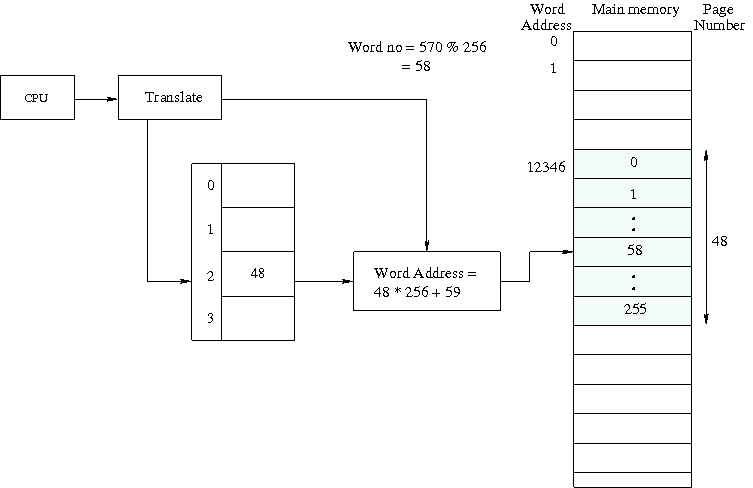
\includegraphics[scale=0.55]{pics/paging_example}
	\caption{Diagram illustrating address translation}
	\label{fig:paging_example}
\end{figure}

\begin{example}
	Consider the scenario in figure~\ref{fig:paging_example}. Here the logical address generated is 570, so the page number is $ \lfloor 570/265 \rfloor = 2$ and word address is $570\mbox{ mod }256 = 58$. The looked up value from the page table is $48$. Thus the resultant physical address is $48 \times 256+58$.
\end{example}
	
\section{Memory Free List}
\label{lbl:memlst}
\index{Memory!Free list}

\begin{itemize}
	\item The free list of the memory consists of 64 entries. Each entry is of size one word.
	\item The total size of the free list is thus 64 words (64 (= no. of entries) $\times$ 1 (= size of one entry) = 64 words).
	\item It is present in the second 64 words of page 2 of the memory. Refer figure~\ref{fig:main memory}.
	\item Each entry of the free list contains a value of either 0 or 1 indicating whether the corresponding page in the memory is free or not respectively.
\end{itemize}

\begin{example} 
	Figure~\ref{fig:mem_free_list} indicates that pages 0, 1 and 63 of the memory are not free while pages 2 and 48 are free.
\end{example}

\begin{figure}[htp!] \small
	\centering
	\begin{tabular}{c|c|}
%		\multicolumn{2}{c}{} \\ 
		\textbf{Pg no.} & \textbf{Contents} \\ \cline{2-2}
		$0$ & $1$ \\ \cline{2-2}
		$1$ & $1$ \\ \cline{2-2}
		$2$ & $0$ \\ \cline{2-2}
		\vdots & \vdots \\ \cline{2-2}
		$48$ & $0$ \\ \cline{2-2}
		$\vdots$ & \vdots \\ \cline{2-2}
		$63$ & $1$ \\ \cline{2-2}
	\end{tabular}
	\caption{A sample free list of the memory}
	\label{fig:mem_free_list}
\end{figure}

The entire structure of memory is outlined in figure~\ref{fig:main memory}.





\begin{itemize}
	\item The ready list is searched for an entry with value 0. The corresponding entry found is set to 1 and the index of this entry is returned as the PID of the process. If no free entry is found, an appropriate error code is returned.
	\item The page table for the process is initialized as follows :
	\begin{enumerate}
		\item The $1^{st}$ entry of the page table contains the page number of the memory where the first code block of the program has been loaded.
		\item The $2^{nd}$ entry of the page table contains the page number of the memory where the second code block of the program has been loaded.
		\item The $3^{rd}$ entry of the page table contains the page number of the memory where the data block of the program has been loaded.
		\item The $4^{th}$ entry of the page table contains the page number of the memory reserved for the stack.
	\end{enumerate}
	\item Set the values of BP, SP and IP in the PCB as 768, 768 and 0 respectively.
	\item Once a process finishes its execution, the entry corresponding to it in the ready list is set to 0.
\end{itemize}


\chapter{Process}
\label{chp:process}
\index{Process}

\section{Introduction}
\begin{defn}
	\textbf{Process :} Any program written by the user is run as a process by the kernel. 
\end{defn}
\begin{itemize}
	\item The {\ESIM} architecture supports a maximum of 12 processes to be run at a time.
	\item Each process occupies 4 pages of the memory.
\end{itemize}

\section{Process Structure}
\index{Process!Structure}
A process in the memory has the following structure.
\begin{itemize}
	\item \textbf{Code Area :} \index{Process!Code Area} These are pages of the memory that contain the actual code to be run on the machine. It occupies 2 pages of the memory. 
	\item \textbf{Data Area :} \index{Process!Data Area} This section consists of string data that is used in the code which cannot be stored in a register. It occupies 1 page of the memory.
	\item \textbf{Stack :} This is the user stack used in program execution. It is used to pass arguments during function calls, storing activation record of a function etc.  It occupies 1 page of the memory and grows in the direction of increasing word address.
\end{itemize}

Figure~\ref{fig:process structure} shows the process structure. \\

\begin{figure}[htp!] 
	\centering
	\begin{tabular}{|c|c} 
		\textbf{Contents}     & \textbf{Pg no:} \\ \cline{1-1}
		\multirow{2}{*}{Code} & $0$ \\
				      & $1$ \\ \cline{1-1}
		Data & 2 \\ \cline{1-1}
		\noalign{\smash{\llap{\lower2pt\hbox{\tt BP$\longrightarrow$}}}}
		&  \\
		&  \\
		\noalign{\smash{\llap{\raise2pt\hbox{\tt $\bigg \downarrow$ }}}}
		Stack & 3 \\ \cline{1-1}
		\noalign{\smash{\llap{\lower2pt\hbox{\tt SP$\longrightarrow$}}}}
	\end{tabular}
	\caption{Process Structure in memory. Arrow shows the direction of stack growth}
	\label{fig:process structure}
\end{figure}

\section{Registers Associated with a Process}
\label{register details}
\begin{itemize}
	\item Every process is allotted a unique integer identifier in the range 0 to 11, known as the PID (Process Identifier) which is stored in the PID register. This register can be used as an operand in any instruction only when executing in the kernel mode. (Refer section~\ref{sec:modes} to know about the modes of operation)
	\index{Registers!PID}
	\item The word address of the currently executing instruction is stored in the IP (Instruction Pointer) register. This register can be used as an operand in any instruction only when executing in the kernel mode.
	\index{Registers!IP}
	\item The base address of the user stack is stored in the BP (Base Pointer) register. \index{Registers!BP}
	\item The address of the stack top is stored in the SP (Stack Pointer) register. \index{Registers!SP}
\end{itemize}
Each process has its own set of values for the various registers.

\section{Data Structures Associated with a Process}
\index{Process Data Structures}

The following are the various data structures associated with a process. They are explained in the following subsections.

\subsection{Ready List}
\index{Process!Ready List}
\label{lbl:rdylst}
The \textit{ready list :} is the data structure that maintains a circular list of all the active processes. Each entry of the ready list contains a value of either 1 or 0 indicating whether the corresponding process in the memory is present in the list or not.

\subsection{Process Control Block (PCB)}
\label{sec:pcb}
\index{Process Data Structures!Process Control Block}
It contains data pertaining to the current state of the process. Refer figure~\ref{fig:PCB}.\\

\newcommand{\pcb}[1]{
	\begin{figure}[htp!]
		\centering
		\begin{tabular}{|c|c|c|c|c|c|}
			\hline
			0 & 1 & 2 & 3 & 4--11 & 12--15 \\
			\hline
			PID & BP & SP & IP & R0 -- R7 & Local File Table \\
			\hline
		\end{tabular}
		\caption{Structure of Process Control Block}
		\label{#1}
	\end{figure}
	}

\pcb{fig:PCB}

Note that the size of each PCB (Process Control Block) is 16 words. 

\subsection{The Page Table}
\label{lbl:pgtbl}
\index{Process!Page Table}
The \emph{page table} stores the exact location in the memory of the data related to a process.
\begin{itemize}
	\item Each process has 4 entries in the page table.
	\begin{itemize}
		\item The zeroth entry corresponds to the first page of code area.
		\item The first entry corresponds to the second page of code area.
		\item The third entry corresponds to the data area.
		\item The fourth entry corresponds to the stack.
	\end{itemize}
	\item Each entry contains the page number where the data specified by the logical address resides in the memory. Refer figure~\ref{fig:paging}.
\end{itemize}

\section{Storage Details of the Data Structures}
	The data structures used by the processes are stored statically in the memory. Their storage details are as follows.\\

\begin{figure}[htp!]
	\centering
	\subfigure[Main Memory]{
	\renewcommand{\arraystretch}{1.2}
	\scalebox{0.85}{
	\begin{tabular}{r|c|} \small
		\textbf{Pg no.} & \textbf{Contents} \\ \cline{2-2}
		0   &  \\ \cline{2-2}
		1   &  \\ \cmidrule{2-2}
		\multirow{4}{*}{2}
			& \cellcolor{gray!70} Static Page Tables   \\ \cline{2-2}
			& Memory Free List     \\ \cline{2-2}
			& Global File Table    \\ \cmidrule{2-2}
			& \cellcolor{cyan!70} Ready List  \\ \cline{2-2}
		3   & \cellcolor{orange!70} Process Table  \\ \cline{2-2}
		    & \vdots \\ \cline{2-2}
		7  &  \\ \cline{2-2}
		\multirow{3}{*}{8 -- 55}
			&  \vdots  \\
			&  User Programs \\
			& \vdots  \\ \cline{2-2}
			&  \\ \cline{2-2}
		56 -- 63 & INT 0 -- 7  \\ \cline{2-2}
		& \vdots   \\ \cline{2-2}
	\end{tabular}}} \\

	\subfigure[Structure of Page Table]{
	\renewcommand{\arraystretch}{1.2}
	\scalebox{0.7}{
	\begin{tabular}{|>{\columncolor[gray]{.8}}c|m{1cm}} \small
		Word Address & Process  \\
		0 & \multirow{4}{*}{$0$}  \\
		1 &  \\
		2 &  \\
		3 &  \\ \cmidrule{1-1}
		\vdots &  \\ \cmidrule{1-1}
		$4i$ & \multirow{4}{*}{$i$}  \\ \cline{1-1}
		$4i+1$ &  \\
		$4i+2$ &  \\
		$4i+3$ &  \\ \cmidrule{1-1}
		\vdots &  \\ \cmidrule{1-1}
		$44$ & \multirow{4}{*}{$11$}  \\
		$45$ &  \\
		$46$ &  \\
		$47$ &  \\
	\end{tabular}}} \qquad \qquad
	\subfigure[Structure of Ready List]{
	\renewcommand{\arraystretch}{1.2}
	\scalebox{0.7}{
	\begin{tabular}{|>{\columncolor{cyan}}c|m{1cm}} \small
		Word Address & Process  \\
		0 & $0$ \\
		1 & $1$ \\
		2 & $2$ \\
		\vdots &  \\
		10 & $10$ \\
		11 & $11$ \\
	\end{tabular}}} \qquad \qquad
	\subfigure[Structure of Process Table]{
	\renewcommand{\arraystretch}{1.2}
	\scalebox{0.7}{
	\begin{tabular}{|>{\columncolor[rgb]{1,0.5,.1}}c|m{1cm}} \small
		Word Address & Process  \\
		0 & \multirow{4}{*}{$0$}  \\
		1 &  \\
		\vdots &  \\
		15 &  \\ \cmidrule{1-1}
		\vdots &  \\ \cmidrule{1-1}
		$16i$ & \multirow{4}{*}{$i$}  \\
		$16i+1$ &  \\
		$16i+2$ &  \\
		\vdots & \\
		$16i+15$ &  \\ \cmidrule{1-1}
		\vdots &  \\ \cmidrule{1-1}
		$176$ & \multirow{4}{*}{$11$}  \\
		$177$ &  \\
		\vdots &  \\
		$191$ &  \\
	\end{tabular}}} \\
	\caption{Data Structures associated with a process}
	\label{fig:ds with process}
\end{figure}

\subsection{Ready List}
\begin{itemize}
	\item The ready list is located in words 209--220 of page 2 of the memory (refer fig~\ref{fig:main memory}).
	\item The size of each ready list entry is one word.
	\item There are a total of 12 processes, thus accounting for the 12 words (12 $\times$ 1 word).
	\item All active processes have an entry 1 in the ready list corresponding to the location indexed by their respective PIDs.
\end{itemize}

\subsection{Page Tables}
\begin{itemize}
	\item The page tables of the 12 processes are stored in the first 48 words of page 2 of the memory. Refer figure~\ref{fig:main memory}.
	\item The size of each page table is 4 words ( 4(= no. of entries) $\times$ 1(= size of an entry)= 4 words).
	\item There are a total of 12 processes, thus accounting for the 48 words( 12 $\times$ 4 words).
	\item The page tables are indexed by multiplying the PID of a process by the size of a page table to get the starting word address of the page table of that process.  The indexing mechanism is illustrated in figure~\ref{fig:ds with process}.
\end{itemize}

\subsection{Process Table}
\index{Process!Process Table}
\label{lbl:proctbl}
\begin{itemize}
	\item The page 3 of the memory contains the process table. Refer figure~\ref{fig:main memory}.
	\item The process table contains the PCB of each of the 12 processes (Each entry occupies 16 words).
	\item There are a total of 12 processes, thus accounting for the 192 words (12 $\times$ 16 words).
	\item The process table is indexed by multiplying the PID of a process by the size of a PCB to get the starting word address of the PCB of that process. The indexing mechanism is illustrated in figure~\ref{fig:ds with process}.
\end{itemize}

\chapter{OS Startup}
\label{chp:osstartup}

\section{ROM Code}
\label{lbl:romcode}
It is a hard coded assembly level code present in page 0 of the memory. Refer figure~\ref{fig:main memory}.
It is also known as the ROM (Read Only Memory) code since in an actual machine it is burnt in the hardware. When the machine boots up, this code is executed. This code has the basic functionality of loading block 0 of the disk (containing the OS startup code) into page 1 of the memory and to set the IP register value to 256 and start execution.

\section{OS Startup Code Specification}
\index{OS Startup Code}
\label{lbl:oscode}
When the machine boots up, the \textit{Bootloader} code loads the \textit{OS startup code} into the main memory. The OS startup code (instructions in page 1, see fig~\ref{fig:main memory}) starts execution in the \textit{Kernel mode}. It performs the following functions.
\begin{itemize}
	\item It loads the Interrupt Service Routines from the blocks 1--8 of the hard disk into pages 56--63 of the memory.
	\item It loads the FAT from blocks 11 and 12 of the hard disk into pages 4 and 5 of the memory.
	\item It loads the disk free list from Blocks 9 and 10 into pages 6 and 7 of the memory.
	\item It generates the memory free list and stores it in words 48--111 of page 2 of the memory.
	\item It loads the INIT process from the hard disk into the memory by performing the following steps:
	\begin{itemize}
		\item Load the INIT process from blocks 14--16 of the hard disk to pages 8--10 of memory. Page 11 is allocated as the user stack.
		\item Update the memory free list.
		\item Update the ready list and PID register.
		\item Set the required page table entries.
		\item Set the values of SP, BP and IP with values 768, 768 and 0 respectively.
	\end{itemize}
	\item Switch from \textit{Kernel mode} to \textit{User mode}.\footnote{This can be achieved by calling IRET.}
\end{itemize}

Note: All addresses are absolute addresses in Kernel mode. 
\section{INIT Process}
\index{INIT Process}
\label{lbl:INITprocess}
The Operating System currently supports execution of only a single user program - the INIT process. Testing of the OS startup code can be done by loading the required user program as the INIT process. Modification to INIT will be done later.

\chapter{Halt System Call}
\label{chp:halt_system_calls}
\index{Halt System Call}

\section{System Calls}
System calls are interfaces through which a process communicates with the OS. Each system call has a unique name associated with it (Halt, Open, Read, Fork etc). Each of these names maps to a unique system call number. Each system call has an interrupt associated with it. Note that multiple system calls can map to the same interrupt.

All the arguments to the system call are pushed as arguments into the user stack while calling the corresponding interrupt. The system call number is pushed as the last argument (Refer section~\ref{callconv} for calling convention).

\section{Halt System Call}
\label{haltsyscall}
\index{File System Calls!Halt}

Syntax : \texttt{Halt()} \\
Syscall no : \counter{syscall} \\

The Halt system call is used to halt the machine. Halt system call invokes the interrupt INT 5. This interrupt consists of a single instruction, the HALT instruction, which halts the simulator.

\chapter{File System Calls}
\label{chp:file_system_calls}
\index{File System Calls}

\section{Scratchpad}
\index{Scratchpad}
There is a specific page of the memory which is reserved to store temporary data. This page is known as the \textit{Scratchpad}. The scratchpad is required since any block of the disk cannot be accessed directly  by a process. It has to be present in the memory for access. Hence, any disk block that has to be read or written into is first brought into the scratchpad. It is then read or modified and written back into the disk (if required).

The page 1 of the memory (fig~\ref{fig:main memory}) is used as the scratchpad. Once the OS has booted up there is no need for the OS startup code. So this page can be reused as the scratchpad.

\section{Global File Table and Local File Table}
Before explaining the system calls, we introduce two data structures : \textit{Global File Table} and \textit{Local File Table}.
\begin{itemize}
	\item \textbf{Global File Table} \label{lbl:gft} \index{Process Data Structures!Global File Table}
	 It is a table consisting of a list of all the open files in the system. Refer fig~\ref{fig:main memory} for location in memory. Since each of the 12 processes can open 4 files at a time, this table consists of a maximum of 48 entries. Each entry of the global file table has the following structure as shown in figure~\ref{fig:gft}.

	 \begin{figure}[h!]
		 \centering
			\begin{tabular}{|c|c|}
				\hline
				FAT Index Entry & lseek\\
				\hline
			\end{tabular}
		 \caption{Structure of a GFT entry}
		 \label{fig:gft}
	 \end{figure}

	 \begin{itemize}
		 \item \textbf{FAT index entry :} \index{File Allocation Table!Memory copy} It is used to index the memory copy of the file allocation table(section~\ref{sec:fat}) to get information about that particular file.

		 \item \textbf{lseek :} It is used to get the current position of the next character that will be read from the file. By default, when a file is opened, this parameter has a value 0.
	 \end{itemize}

	\item \textbf{Local File table} \label{lbl:lft} \index{Process Data Structures!Local File Table}
	In addition to the fields discussed earlier(section~\ref{sec:pcb}), the PCB has an additional field known as the \emph{Local File Table}. The local file table consists of 4 entries each of size one word. Each entry corresponds to a file opened by that particular process and stores the global file table index of that file. Thus a process can open a maximum of 4 files. 
	
	The local file table is indexed by a \textit{file descriptor}(an integer value ranging from 0 to 3).
\end{itemize}

\section{Modifications in the OS Startup Code}
\begin{itemize}
	\item The Global File Table in the memory must be initialised with NULL values.

	\item The Local File Table entries in the PCB of the INIT process must be initialised with NULL values.
\end{itemize}

\section{File System Calls}
\label{fssyscall}
\textit{File system calls} are used by a process when it has to create, delete or manipulate \textit{Data files} that reside on the disk(file system). There are seven file system calls. An interrupt is associated with each system call. All the necessary arguments for a system call are available in the user stack with the system call number as the last argument.\\

\noindent Interrupt specifications for different \textit{File system calls} are as follows:

\subsection{INT 1}
The file system calls \textit{Create} and \textit{Delete} invoke INT 1. INT 1 handles these system calls as follows.
\begin{enumerate}
	\item  \textbf{Create :} This system call is used to create a new file in the file system whose name is specified in the argument.\\
	Syntax : \texttt{int Create(fileName)} \\
	Syscall no : \counter{syscall}
	\index{File System Calls!Create}
	\begin{itemize}
		\item First of all, the memory copy of the FAT \index{File Allocation Table!Memory copy} is searched for a free entry. If no free entry is found, an appropriate error code is returned.
		
		\item Next, the memory copy of the disk free list \index{Disk Free List!Memory copy} is searched to find a free block number.If no free block is found, an appropriate error code is returned. This block is used as the basic block of the file to be created.
		
		\item The \texttt{fileName} specified in the argument and the free block number obtained in the previous step are stored in the \emph{file name} field and \emph{basic block number} field of the free FAT entry, respectively.
				
		\item The \emph{file size} field of the FAT entry is initialized to zero.
		
		\item Each entry of the block list in the basic block is initialized to zero.\footnote{This can be achieved by loading the basic block into the scratchpad, updating it and then committing back the updated basic block.}
		
		\item The updated copies of FAT \index{File Allocation Table!Memory copy} and disk free list 
		\index{Disk Free List!Memory copy} in the memory are committed to the disk.
		
		\item The return value of this system call is 0 in case of success and the appropriate error code in case of failure.
	\end{itemize}

	\item \textbf{Delete :} This system call is used to delete the file from the file system whose name is specified in the argument. \\
	Syntax : \texttt{int Delete(fileName)} \\
	Syscall no : \counter{syscall}
	\index{File System Calls!Delete}
	\begin{itemize}
		\item The memory copy of the FAT \index{File Allocation Table!Memory copy} is searched using the \texttt{fileName} to get the corresponding FAT entry. If no entry is found, an appropriate error code is returned.
		
		\item If the file is already open an appropriate error code is returned. We adopt the following steps to check if the file is open.
		\begin{itemize}
			\item The \emph{FAT index entry} of each global file table entry is used to fetch the filename of the corresponding open file from the memory copy of the FAT \index{File Allocation Table!Memory copy}.
			
			\item Each of the filenames obtained in the previous step is compared with the \texttt{fileName}. If match is found, we conclude that the file is currently in open.
		\end{itemize}
		\item The \emph{basic block number} field in this FAT entry obtained, is then used to load the basic block of the file into the scratchpad.
		
		\item Each entry in the block list of the basic block is used to find the data blocks of the file. Then, entries in the memory copy of the disk free list \index{Disk Free List!Memory copy}  corresponding to these data blocks are set to zero, thereby freeing them.
		
		\item Finally, the FAT entry of the file is removed.
		
		\item The updated copies of FAT \index{File Allocation Table!Memory copy} and disk free list \index{Disk Free List!Memory copy} in the memory are committed to the disk.
		
		\item The return value of this system call is 0 in case of success and the appropriate error code in case of failure.
	\end{itemize}
\end{enumerate}

\subsection{INT 2}
The file system calls \textit{Open} and \textit{Close} invoke INT 2. INT 2 handles these system calls as follows.
\begin{enumerate}
	\item \textbf{Open :} This system call is used to open an existing file whose name is specified in the argument.\\
	Syntax : \texttt{int Open(fileName)} \\
	Syscall no : \counter{syscall} 
	\index{File System Calls!Open}
	\begin{itemize}
		\item  First of all, a free entry is searched in the local file table of the process. If there are no free entries, in the case where a process already has 4 open files, an appropriate error code is returned.
		
		\item Then, the global file table is searched for a free entry. If there is no free entry, an appropriate error code is returned else a new global file table entry is created and the fields are filled with appropriate values in the following manner:
		\begin{itemize}
			\item The memory copy of FAT \index{File Allocation Table!Memory copy} is searched using the \texttt{fileName} and the corresponding index of that file in the FAT \footnote{By index, we mean the sequential position (starting from 0) of that entry in the data structure mentioned.} is stored as the \emph{FAT index}. If the file does not have an entry in the FAT, an appropriate error code is returned.
			
			\item The \emph{lseek} field is set to zero.
		\end{itemize}
		
		\item The index of this global file table entry is stored in its local file table.
		
		\item The index of this entry in the local file table is returned as a return value of the system call. This is known as the file descriptor.
	\end{itemize}

	\item  \textbf{Close :} This system call is used to close an open file. The file can only be closed by the process which opened it or by its children. \\
	Syntax : \texttt{int Close(fileDescriptor) } \\
	Syscall no : \counter{syscall}
	\index{File System Calls!Close}
	\begin{itemize}
		\item The \texttt{fileDescriptor} is used first to access the local file table entry of the file. An appropriate error code is returned if the \texttt{fileDescriptor} is out of the range specified.
		
		\item The global file table entry indexed by this local file table entry is removed. \footnote{A suggested way to remove an entry is to store an integer -1 in that word.} %TODO -1 or ''\0``
		
		\item The local file table entry of the process is then removed.
		
		\item The return value of this system call is 0 in case of success and the appropriate error code in case of failure.
	\end{itemize}
\end{enumerate}

\subsection{INT 3}
The file system calls \textit{Read} and \textit{Seek} invoke INT 3. INT 3 handles these system calls as follows.
\begin{enumerate}
	\item \textbf{Seek :} This system call is used to change the current value of the seek position in the global file table entry of a file. \\
	Syntax : \texttt{int Seek(fileDescriptor, lseek)}  \\
	Syscall no : \counter{syscall}
	\index{File System Calls!Seek}
	\begin{itemize}
		\item The \texttt{fileDescriptor} is used first to access the local file table entry of the file. An appropriate error code is returned if the \texttt{fileDescriptor} is out of the range specified.
		\item This local file table entry is then used to access the global file table entry of the file.
		\item Then the FAT index field in the global file table entry is used to access the FAT entry of the file.
		\item The \emph{file size} got from this FAT entry is checked to be greater than \texttt{lseek}. Otherwise an appropriate error code is returned.\footnote{Seek is allowed only \emph{within} a file.}
		\item The \emph{lseek} field in the GFT entry is then changed to the new value specified in the argument (\texttt{lseek}).
		\item The return value of this system call is 0 in case of success and the appropriate error code in case of failure.
	\end{itemize}
	
	\item \textbf{Read :} This system call is used to read data from an open file.\\
	Syntax : \texttt{int Read(fileDescriptor, mem\_loc, numWords)} \\
	Syscall no : \counter{syscall}
	\index{File System Calls!Read}
	\begin{itemize}
		\item First of all, the basic block of the file specified by the \texttt{fileDescriptor} is loaded in the scratchpad. This is done in the following way:
		\begin{itemize}
			\item The \texttt{fileDescriptor} is used first to access the local file table entry of the file. An appropriate error is returned if the \texttt{fileDescriptor} is out of the range specified.
			\item This local file table entry is then used to access the global file table entry of the file. 
			\item Then the \emph{FAT index} field in the global file table entry is used to access the FAT entry of the file.
			\item The basic block address present in the FAT entry is then used to load the basic block (containing block list and file header info) into the scratchpad. Refer figure~\ref{access_scheme}.
		\end{itemize}	
		\item The \emph{lseek} position present in the GFT entry and \texttt{numWords} are used to index the block list in the basic block to find the address of the block(s) to be read.
		\item Each time the block to be read is loaded into the scratchpad before reading its contents.
		\item The contents read are then copied into the buffer that is specified as an argument to the system call (\texttt{mem\_loc}). If the \texttt{mem\_loc} is out of the address space of the process, an appropriate error code is returned.
		\item The return value of this system call is the number of words successfully read. In case of an error, an appropriate error code is returned.
	\end{itemize}
\end{enumerate}

\begin{figure}[htp!]
	\centering
	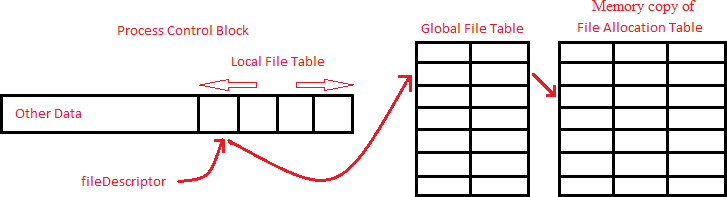
\includegraphics[scale=0.65]{pics/access_method}
	\caption{Diagram showing the method of accessing FAT entry}
	\label{access_scheme}
\end{figure}

\subsection{INT 4}
The file system call \textit{Write} invoke INT 4. INT 4 handles these system calls as follows.

\textbf{Write :} This system call is used to write data into an open file. \\
Syntax : \texttt{int Write(fileDescriptor, mem\_loc, numWords)} 
\footnote{It is advisable to have  a maximum of 1 block for any data file if it has to be modified using \texttt{write} system call since if the modification spans multiple blocks the entire procedure to access a block (outlined above) has to be repeated.} \\
Syscall no : \counter{syscall}
\index{File System Calls!Write}
\begin{itemize}
	\item First of all, the basic block of the file specified by the \texttt{fileDescriptor} is loaded into the scratchpad. This is done in the following way:
	\begin{itemize}
		\item The \texttt{fileDescriptor} is used first to access the local file table entry of the file. An appropriate error is returned if the \texttt{fileDescriptor} is out of the range specified.
		\item This local file table entry is then used to access the global file table entry of the file.
		\item Then the FAT index field in the global file table entry is used to access the FAT entry of the file.
		\item The basic block address present in the FAT entry is then used load the basic block (containing block list and file header info) into the scratchpad. Refer figure~\ref{access_scheme}.
	\end{itemize}	
	
	\item The lseek position present in the GFT entry and \texttt{numWords} are used to index the block list in the basic block to find the block numbers of the block(s) to be written into. \footnote{The data block to which the lseek position is pointing to is got by dividing lseek by the block size. \\
	The data block number calculated above is used to index the block list in the basic block to get the exact location of the data block in the disk. The data block is then loaded from the disk into the scratchpad. \\
	If the words to be read are split across multiple data blocks, the above procedure is repeated.}
	
	\item Each time the block to be written into is loaded into the scratchpad before performing the write operation.
	
	\item After loading the specified block, the content to be written is copied from the user memory location (\texttt{mem\_loc}) into this block. If \texttt{mem\_loc} is out of the address space of the process, an appropriate error code is returned.
	
	\item If the write operation exhausts all the currently allocated blocks, new blocks are allocated as required. This is done in the following way.
	\begin{itemize}
		\item The memory copy of the disk free list \index{Disk Free List!Memory copy} is used to get the block number of a free block.
		\item A new basic block entry is created using this free block number and added to the block list of the basic block. Successive write operations are then performed the usual way.
	\end{itemize}
	
	\item Once all the write operations are over for that block, it is stored back into the disk.
	
	\item The updated copies of FAT \index{File Allocation Table!Memory copy} and disk free list 
	\index{Disk Free List!Memory copy} in the memory are committed to the disk.
	
	\item The return value of this system call is the number of words successfully written. In case of an error, an appropriate error code is returned.
\end{itemize}

\chapter{Multiprogramming}
\label{chp:multiprog}
To support multiprogramming in the system, the kernel makes use of the \emph{scheduler} which is present in the interrupt service routine INT 0\footnote{Unlike other interrupts, INT 0 is called by the machine and not by the user program.}.

\section{Scheduler}
\label{chp:scheduler}
\index{Scheduler}
Whenever a timer interrupt occurs, the kernel temporarily halts the execution of the currently executing process and invokes INT 0.
Refer book~\cite{Crowley} for more details.
Following are functionalities of the scheduler:
\begin{itemize}
	\item If a process is currently running, the scheduler saves the values of all the registers into the corresponding fields in the PCB of that process.
	\item The scheduler scans the ready list starting from the current PID and checks for the presence of a process other than the INIT process.\footnote{This can be accomplished by setting the PID of INIT process as 0 and searching only the entries from 1--11 in the ready list.} If one such process is found, the PID is updated with the index of this entry in the ready list. If no such process is found, then the PID is set to the index of the INIT process in the ready list. Then all the registers of the machine are initialised with their corresponding values obtained from the PCB of the process specified by this PID.
	\item The process switches from \textit{Kernel mode} to \textit{User mode}.
\end{itemize}

\chapter{Process System Calls}
\label{chp:process_system_calls}
\index{Process System Calls}

\section{Process System Calls}
\label{procsyscall}
\index{Process System Calls}
\textit{Process system calls} are used by a process when it has to duplicate itself, execute a new process in its place or when it has to terminate itself. There are three process system calls. An interrupt is associated with each system call. All the necessary arguments for a system call are available in the user stack with the system call number as the last argument.\\

\noindent Interrupt specifications for different \textit{Process system calls} are as follows:

\subsection{INT 5}
The process system call \textit{Fork} invokes INT 5. INT 5 handles these system calls as follows.

\textbf{Fork :}  This system call is used to create a new process having the same code area, data area and list of open files as that of the process which invoked this system call.

The new process that is created is known as the \emph{child} process, and the process which invoked this system call is known as its \emph{parent}.

The register values in the PCB of the child process are initialized with the current register contents.\\
Syntax : \texttt{int Fork()} \\
Syscall no : \counter{syscall}
\index{Process System Calls!Fork}
\begin{itemize}
	\item A vacant entry is searched for in the \emph{Ready list}.
	\item If no entry is found, in the case when there are already 12 processes that are active, an appropriate error code is returned.
	\item The index of this vacant ready list entry is the PID for the child process that is created.
	\item The PID entry in the PCB of the child process is updated with this new PID.
	\item All the registers (except PID) and the local file table of the parent process is replicated in the PCB of the child process.
	\item The code pages, the data page and the stack page of the parent process is replicated for this child process.
	\item The control is returned back to the parent process.
	\item The return value of this system call is the PID of the child process.
\end{itemize}

\subsection{INT 6}
The process system call \textit{Exec} invokes INT 6. INT 6 handles these system calls as follows.

\textbf{Exec :}  This system call is used to load the program, whose name is specified in the argument, in the memory space of the current process and start its execution .\\
Syntax : \texttt{int Exec(filename)} \\
Syscall no : \counter{syscall}
\index{Process System Calls!Exec}
\begin{itemize}
	\item The entire process area of the currently executing process is replaced by that of the program specified in the argument (\texttt{filename}). 
	\item If the file specified by \texttt{filename} is not an executable \footnote{Executables in {\ESIM} must end with an extension \texttt{.sim}} then, an appropriate error code is returned.
	\item The memory copy of the FAT \index{File Allocation Table!Memory copy} is searched to get the location of the basic block of the file specified by \texttt{filename}, which is then loaded into the scratchpad.
	\item This is then used to get the location in the disk of the blocks of the file to be loaded.
	\item The 2 code blocks and 1 data block of the file are loaded from the disk into the corresponding locations in the memory of the code blocks and data block of the current process.
	\item The PCB of the current process is modified to hold the values for that of the new process. The PID and page table, however, remains unchanged.\footnote{This is because the mappings remain the same as the code blocks and data block of the specified executable are loaded into the same locations as of the current process. Since, no new process table entry is created, the PID also remains the same.}
	\item The return value of this system call is 1 in case of a failure. Nothing is returned in case of a success.
\end{itemize}

\subsection{INT 7}
The process system call \textit{Exit} invokes INT 7. INT 7 handles this system call as follows.
\textbf{Exit :}  This system call is used to terminate the execution of the process which invoked it and removes it from the memory . It loads the next available process.\\
Syntax :  \texttt{Exit()}  \\
Syscall no : \counter{syscall}
\index{Process System Calls!Exit}
\begin{itemize}
	\item The entire address space of the currently executing process is set free by setting a value 0 in the memory free list corresponding to the pages occupied by that process.
	
	\item The local file table is traversed and the global file table entry is removed.
	
	\item The ready list entry corresponding to this process is set to zero thereby releasing all the data structures used by the process (fig~\ref{fig:ds with process}).
	
	\item The ready list is then searched for the next available process. The INIT process is excluded in this search.\footnote{This can be accomplished by setting the PID of INIT process as 0 and searching only the entries from 1--11 in the ready list.} If one such process is found, the PID is updated with the index of this entry in the ready list. If no such process is found, then the PID is set to the index of the INIT process in the ready list.
	
	\item All the registers of the machine are initialised with their corresponding values obtained from the PCB of the process specified by the new PID.
	
	\item The process switches from \textit{Kernel mode} to \textit{User mode}.
\end{itemize}

\section{INIT Process}
The INIT process is the first user process loaded by the OS on the OS startup. INIT was previously defined in chapter~\ref{chp:osstartup} as a normal user program. Since multiprogramming functionalities have been added to the OS, INIT must be modified. The modified specification of INIT process is as follows:
\begin{itemize}
	\item  It provides an interface for the users to run other user programs.
	\item The user enters the name of a valid executable file (which should be made available in the disk) in the shell. If the specified file is not found, an appropriate error code is returned.
	\item If the specified executable file is found, the INIT process forks and does exec on the that file.
	\item Entering the keyword HALT instead of the name of an executable file invokes the Shutdown system call.
\end{itemize}

All the user processes other than INIT are added to entries 1-11 of the ready queue keeping the 0th entry (corresponding to INIT) untouched. INIT loads the first process and thereafter all context switches occur among the other processes in the ready queue. INIT is switched back only when the ready queue (entries 1-11) is free so that the user can load another executable file via the shell. 

%\appendix TODO !!
%\section{Simple Integer Machine (SIM) architecture}
% \chapter{System Programmer's manual}
% The following diagram illustrates the interaction among various modules that have been written in the code. 
% 
%  \begin{figure}[htp!]
% 	  \centering
% % 	  \includegraphics[scale=0.55]{pics/spm}
% 	  \caption{Interaction among various modules in the implementation}
% 	  \label{fig:spm}
% 	  \end{figure}
% 
% Each module performs a specific function which has been well documented in the code. All variables and data structures that are used are suitably named and proper constants have been defined for anything that has a fixed value like location in memory of the various data structures and other machine constants. 



\end{document}